\section*{Evaluation}
\label{sec:evaluation}

\begin{figure*}[ht]
\centering
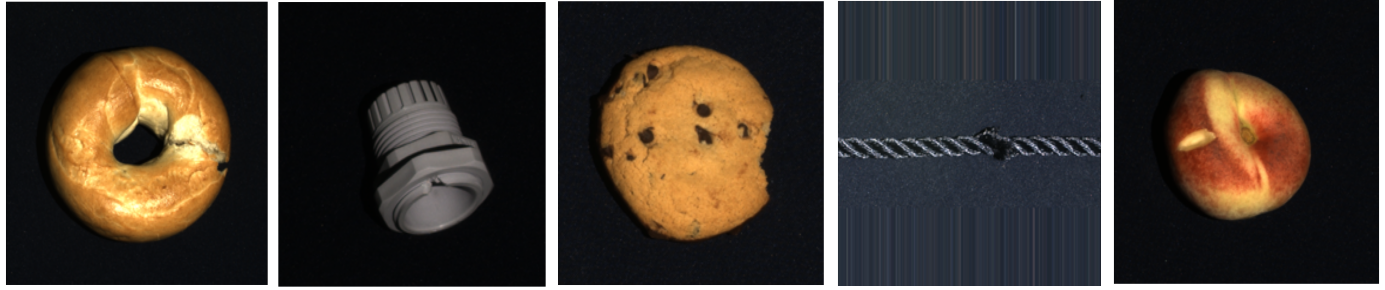
\includegraphics[width=\linewidth]{figs/result_rgb}
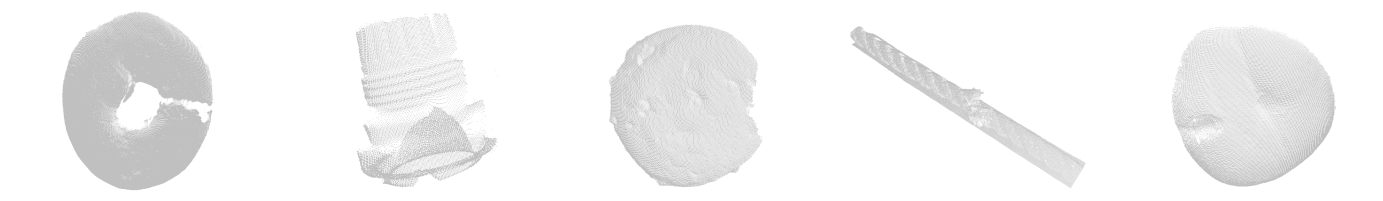
\includegraphics[width=\linewidth]{figs/result_pc}
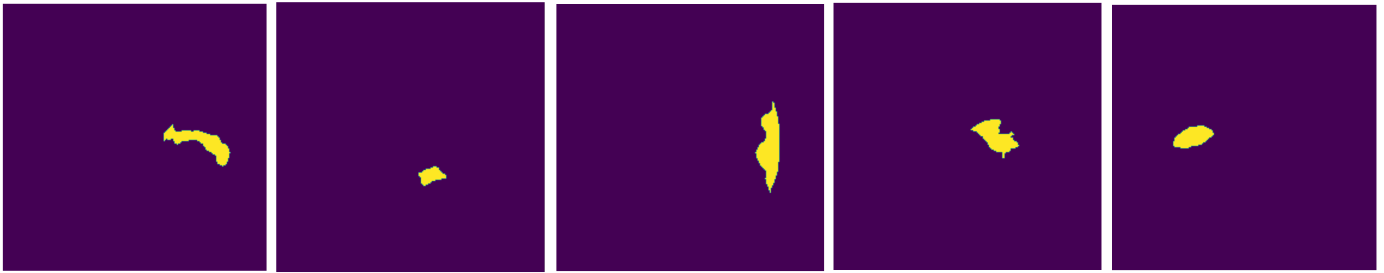
\includegraphics[width=\linewidth]{figs/result_gt}
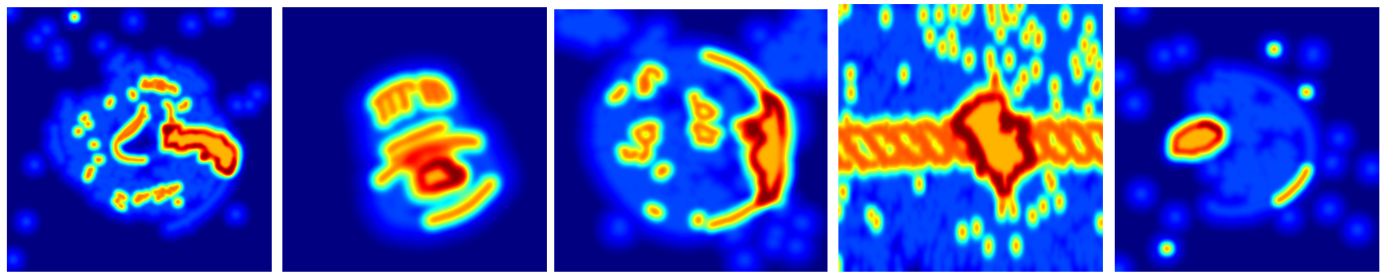
\includegraphics[width=\linewidth]{figs/result_baseline}
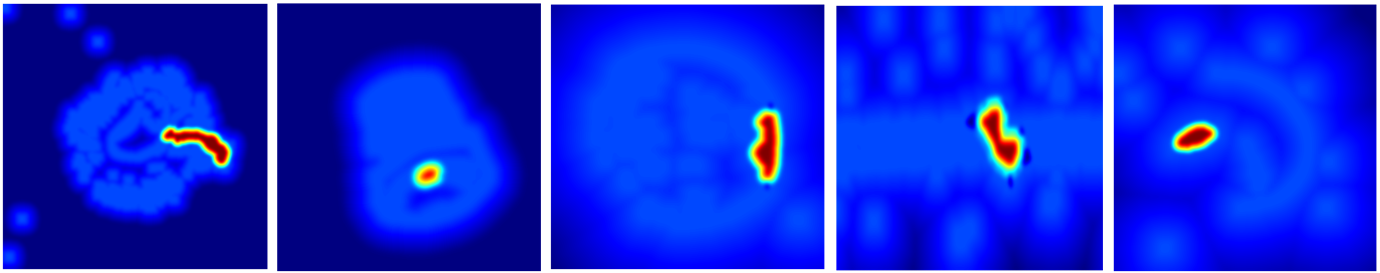
\includegraphics[width=\linewidth]{figs/result_ours}
\caption{Qualitative results of anomaly detection. From top to bottom: input RGB images, point clouds, ground-truth anomaly segmentations, anomaly maps from \cite{wang2023multimodal}, and anomaly maps obtained with our proposed method.}
\label{fig:results}
\end{figure*}

\subsection*{Experimental Details}

\textbf{Dataset.}  Most existing industrial anomaly detection datasets provides 2D RGB images without corresponding 3D point cloud data. In contrast, 3D industrial anomaly detection is still in its early stages. The MVTec 3D-AD dataset \cite{bergmann2022mvtec} is the first 3D dataset for industrial anomaly detection. Following previous works \cite{wang2023multimodal}, we conduct our experiments on this dataset, which is designed to reflect real-world industrial inspection scenarios. The dataset includes 10 categories of industrial objects, comprising 2656 training samples, 294 validation samples, and 1197 test samples. The 3D scans were captured using a structured light-based industrial sensor, where the position information is stored in three-channel tensors representing x, y, and z coordinates. Each sample includes both RGB images and pixel-registered 3D information, providing a rich dataset for experiments. The object categories vary from items with natural variations (e.g., bagels, carrots, peaches) to more rigid and structured items (e.g., cable glands, dowels). The test set contains simulated real-world defects such as scratches, dents, holes, contaminations, and deformations, with ground-truth annotations provided for each anomalous sample. \\

\noindent \textbf{Implementation Details.} Following \cite{wang2023multimodal}, we apply the RANSAC algorithm \cite{fischler1981random} to estimate the background plane, discarding any points within a distance of 0.005 units. For feature extraction, we utilize frozen Transformers as in \cite{wang2023multimodal}. Specifically, we employ DINO ViT-B/8 \cite{dosovitskiy2020image} pre-trained on ImageNet \cite{deng2009imagenet} for visual feature extraction, and Point-MAE \cite{pang2022masked} pre-trained on ShapeNet \cite{chang2015shapenet} for geometric feature extraction. The visual feature extraction module processes RGB images of resolution $224 \times 224$, producing a $28 \times 28 \times 768$ feature map, which is then upsampled to $224 \times 224 \times 768$ using bilinear interpolation before being passed to the geometric feature reconstruction module. For the point cloud data, we sample 1024 groups of 32 points using Farthest Point Sampling (FPS) \cite{qi2017pointnet++}, yielding a $1152$-dimensional feature vector for each group. These feature vectors are interpolated and aligned to a $224 \times 224 \times 1152$ grid, which serves as the target geometric feature map for reconstruction. The geometric feature reconstruction module is composed of three fully connected layers with GeLU activation functions applied after the first two layers. The layers have 768, 960, and 1152 units, respectively. We train the network for 200 epochs using the Adam optimizer \cite{kingma2014adam} with a learning rate of 0.001. All experiments are conducted on a single NVIDIA GeForce RTX 4090 GPU, utilizing both our implementation and the original authors' code for comparison. \\

\noindent \textbf{Evaluation Metrics.} Following \cite{bergmann2022mvtec, wang2023multimodal}, we employ two metrics: the Image-level Area Under the Receiver Operating Characteristic curve (I-AUROC) and the Area Under the Per-Region Overlap curve (AUPRO). These metrics provide insights into both anomaly classification and localization performance. I-AUROC is used to assess the model's ability to classify an entire test image as either anomaly-free or containing an anomaly. The AUROC curve is derived by plotting the true positive rate (TPR) against the false positive rate (FPR) at various threshold levels. The I-AUROC score provides a threshold-independent evaluation of the model's classification performance, with a score of 1 indicating perfect classification. A higher I-AUROC score signifies better image-level anomaly detection performance. AUPRO evaluates the model's ability to localize anomalies within the test samples. AUPRO measures how well the predicted anomaly regions overlap with the ground truth at different thresholds, thus reflecting the model's localization accuracy. For each connected component \( C_k \) in the ground truth, the overlap between the binary prediction \( P \) and \( C_k \) is computed. The Per-Region Overlap (PRO) for each region is defined as:
\begin{equation}
    \text{PRO}(C_k) = \frac{|P \cap C_k|}{|C_k|}
\end{equation}
AUPRO is computed by integrating the PRO over a range of thresholds, typically up to a false positive rate (FPR) limit.  We report the area under the PRO curve with an upper integration limit of 0.3 as in \cite{bergmann2022mvtec}. By focusing on localization performance, AUPRO offers a more precise evaluation of anomaly detection in complex industrial settings, where accurately pinpointing defect regions is critical. These metrics together provide a comprehensive view of the model's ability to detect and localize anomalies.

\subsection*{Results}

\begin{table*}[ht]
\centering
\begin{tabular}{cl|r|r|r|r|r|r|r|r|r|r|r}
\hline
& Method & Bagel & \makecell{Cable \\ Gland} & Carrot & Cookie & Dowel & Foam & Peach & Potato & Rope & Tire & Mean \\
\hline
\parbox[t]{0.5mm}{\multirow{8}{*}{\rotatebox[origin=c]{90}{3D}}} & Depth GAN & 0.530 & 0.376 & 0.607 & 0.603 & 0.497 & 0.484 & 0.595 & 0.489 & 0.536 & 0.521 & 0.523 \\
& Voxel AE & 0.693 & 0.425 & 0.515 & 0.790 & 0.494 & 0.558 & 0.537 & 0.484 & 0.639 & 0.583 & 0.571 \\
& Depth AE & 0.468 & 0.731 & 0.497 & 0.673 & 0.534 & 0.417 & 0.485 & 0.549 & 0.564 & 0.546 & 0.546 \\
& Voxel VM & 0.750 & 0.747 & 0.613 & 0.738 & 0.823 & 0.693 & 0.679 & 0.652 & 0.609 & 0.690 & 0.699 \\
& Depth VM & 0.510 & 0.542 & 0.469 & 0.576 & 0.609 & 0.699 & 0.450 & 0.419 & 0.668 & 0.520 & 0.546 \\
& FPFH & 0.825 & 0.551 & 0.952 & 0.797 & 0.883 & 0.582 & 0.758 & 0.889 & 0.929 & 0.653 & 0.782 \\
& Voxel GAN & 0.383 & 0.623 & 0.474 & 0.639 & 0.564 & 0.409 & 0.617 & 0.427 & 0.663 & 0.577 & 0.537 \\
& AST & 0.881 & 0.576 & 0.965 & 0.957 & 0.679 & 0.797 & \textbf{0.990} & 0.915 & 0.956 & 0.611 & 0.833 \\
& 3D-ST & 0.862 & 0.484 & 0.832 & 0.894 & 0.848 & 0.663 & 0.763 & 0.687 & 0.958 & 0.486 & 0.748 \\
& M3DM & 0.941 & 0.651 & 0.965 & 0.969 & 0.905 & 0.760 & 0.880 & 0.974 & 0.926 & 0.765 & 0.874 \\
\hline
\parbox[t]{0.5mm}{\multirow{3}{*}{\rotatebox[origin=c]{90}{RGB}}} & DifferNet & 0.859 & 0.703 & 0.643 & 0.435 & 0.797 & 0.790 & 0.787 & 0.643 & 0.715 & 0.590 & 0.696 \\
& STFPM & 0.930 & 0.847 & 0.980 & 0.575 & 0.947 & 0.766 & 0.710 & 0.598 & 0.965 & 0.701 & 0.793 \\
& PADiM & 0.975 & 0.775 & 0.698 & 0.582 & 0.663 & 0.582 & 0.660 & 0.535 & 0.832 & 0.760 & 0.764 \\
& AST & 0.947 & \textbf{0.928} & 0.851 & 0.825 & \underline{0.981} & \underline{0.951} & 0.895 & 0.613 & 0.992 & 0.821 & 0.880 \\
& PatchCore & 0.876 & 0.880 & 0.791 & 0.682 & 0.912 & 0.701 & 0.695 & 0.618  & 0.841 & 0.702 & 0.770 \\
& M3DM & 0.944 & 0.918 & 0.896 & 0.749 & 0.959 & 0.767 & 0.919 & 0.648 & 0.938 & 0.767 & 0.850 \\
\hline
\parbox[t]{0.5mm}{\multirow{8}{*}{\rotatebox[origin=c]{90}{RGB + 3D}}} & Depth GAN & 0.538 & 0.372 & 0.580 & 0.603 & 0.430 & 0.534 & 0.042 & 0.601 & 0.443 & 0.577 & 0.532 \\
& Voxel AE & 0.510 & 0.540 & 0.384 & 0.693 & 0.632 & 0.550 & 0.494 & 0.721 & 0.413 & 0.538 & 0.538 \\
& Depth AE & 0.648 & 0.502 & 0.650 & 0.488 & 0.805 & 0.522 & 0.712 & 0.529 & 0.540 & 0.552 & 0.595 \\
& Voxel VM & 0.553 & 0.772 & 0.484 & 0.701 & 0.751 & 0.578 & 0.480 & 0.466 & 0.689 & 0.611 & 0.609 \\
& Depth VM & 0.513 & 0.551 & 0.477 & 0.581 & 0.617 & 0.716 & 0.450 & 0.421 & 0.598 & 0.623 & 0.555 \\
& AST & 0.983 & 0.873 & 0.976 & 0.971 & 0.932 & 0.885 & 0.974 & 0.981 & \textbf{1.000} & 0.797 & 0.937 \\
& Voxel GAN & 0.680 & 0.324 & 0.565 & 0.509 & 0.599 & 0.579 & 0.601 & 0.482 & 0.601 & 0.482 & 0.517 \\
& 3D-ST & 0.950 & 0.483 & \underline{0.986} & 0.921 & 0.905 & 0.632 & 0.945 & \textbf{0.988} & 0.976 & 0.542 & 0.833 \\
& M3DM & \textbf{0.994} & 0.909 & 0.972 & \underline{0.976} & 0.960 & 0.942 & 0.973 & 0.899 & 0.972 & \underline{0.850} & \underline{0.945} \\
& Ours & \underline{0.990} & \underline{0.922} & \textbf{0.988} & \textbf{0.979} & \textbf{0.984} & \textbf{0.973} & \underline{0.988} & \underline{0.985} & \underline{0.994} & \textbf{0.883} & \textbf{0.968} \\
\hline
\end{tabular}
\caption{\label{tab:1} I-AUROC score for anomaly detection of all categories of MVTec-3D AD. Results FPFH \cite{horwitz2022empirical}, PatchCore \cite{roth2022towards}, PADiM \cite{defard2021padim}, 3D-ST \cite{bergmann2023anomaly}, AST \cite{rudolph2023asymmetric}, DifferNet \cite{rudolph2021same}, STFPM \cite{wang2021student}, M3DM \cite{wang2023multimodal} are obtained from \cite{wang2023multimodal}, and the remaining methods from \cite{bergmann2022mvtec}. Best results in \textbf{bold}, runner-ups \underline{underlined}.}
\end{table*}
%/--------------------------------------------------------------------

Figure \ref{fig:results} demonstrates the qualitative performance of our method on the MVTec 3D-AD dataset. In comparison to the baseline, our anomaly maps exhibit significantly sharper localization, aligning closely with the ground-truth defect regions. Table \ref{tab:1} presents the I-AUROC scores for various anomaly detection methods evaluated on the MVTec-3D AD dataset. The proposed method demonstrates good performance across most categories, achieving the highest mean I-AUROC score of 0.968. This performance highlights the model's superior ability to differentiate between normal and anomalous samples. The key reason behind this success lies in the visual-to-geometric feature reconstruction approach, which allows the model to predict geometric features from visual features, thereby learning complex correlations between appearance and structure in normal objects. In comparison to other methods, such as AST \cite{rudolph2023asymmetric} and M3DM \cite{wang2023multimodal}, the proposed model consistently outperforms in many object categories, including ``Cookie," ``Dowel," ``Foam," and ``Tire," achieving scores of 0.979, 0.984, 0.973, and 0.883, respectively. These high scores demonstrate the efficacy of the Visual-to-Geometric Feature Reconstruction network, which effectively learns the correlation between 2D visual features and 3D geometric features, allowing the model to be highly responsive to irregularities in both the appearance and structure of objects. However, the proposed method does not always perform better than certain RGB-only methods. For instance, in the ``Cable Gland" category, the proposed method achieves an I-AUROC score of 0.922, whereas the RGB-based AST model attains a slightly higher score of 0.928. This discrepancy might be attributed to the nature of the cable gland object, which is characterized by complex geometry and reflective surfaces that can be difficult to accurately measure in 3D. The presence of intricate details and curved surfaces introduces noise and inaccuracies in the 3D point cloud data, leading to suboptimal feature reconstruction and anomaly detection. The RGB-only models, such as AST, is benefit in this case from focusing solely on visual information without the added complexity of geometric features, which might not be reliably captured.

%/--------------------------------------------------------------------
\begin{table*}[ht]
\centering
\begin{tabular}{cl|r|r|r|r|r|r|r|r|r|r|r}
\hline
& Method & Bagel & \makecell{Cable \\ Gland} & Carrot & Cookie & Dowel & Foam & Peach & Potato & Rope & Tire & Mean \\
\hline
\parbox[t]{0.5mm}{\multirow{8}{*}{\rotatebox[origin=c]{90}{3D}}} & Depth GAN & 0.111 & 0.072 & 0.212 & 0.174 & 0.160 & 0.128 & 0.003 & 0.042 & 0.446 & 0.075 & 0.143 \\
& Voxel AE & 0.260 & 0.341 & 0.581 & 0.351 & 0.502 & 0.234 & 0.351 & 0.658 & 0.015 & 0.185 & 0.348 \\
& Depth AE & 0.147 & 0.069 & 0.293 & 0.217 & 0.207 & 0.181 & 0.164 & 0.066 & 0.545 & 0.142 & 0.203 \\
& Voxel VM & 0.453 & 0.343 & 0.521 & 0.697 & 0.680 & 0.284 & 0.349 & 0.634 & 0.616 & 0.346 & 0.492 \\
& FPFH & 0.973 & 0.879 & 0.982 & 0.906 & 0.892 & 0.735 & \underline{0.977} & 0.982 & 0.956 & 0.961 & 0.924 \\
& Depth VM & 0.280 & 0.374 & 0.243 & 0.526 & 0.485 & 0.314 & 0.199 & 0.388 & 0.543 & 0.385 & 0.374 \\
& Voxel GAN & 0.440 & 0.453 & 0.875 & 0.755 & 0.782 & 0.378 & 0.392 & 0.639 & 0.775 & 0.389 & 0.583 \\
& M3DM & 0.943 & 0.818 & 0.977 & 0.882 & 0.881 & 0.743 & 0.958 & 0.974 & 0.950 & 0.929 & 0.906 \\
\hline
\parbox[t]{0.5mm}{\multirow{4}{*}{\rotatebox[origin=c]{90}{RGB}}} & CFlow & 0.855 & 0.919 & 0.958 & 0.867 & 0.969 & 0.500 & 0.889 & 0.935 & 0.904 & 0.919 & 0.871 \\
& PADiM & \textbf{0.980} & 0.944 & 0.945 & 0.925 & 0.961 & 0.792 & 0.966 & 0.940 & 0.937 & 0.912 & \textbf{0.930} \\
& PatchCore & 0.901 & 0.949 & 0.928 & 0.877 & 0.892 & 0.563 & 0.904 & 0.932 & 0.908 & 0.906 & 0.876 \\
& M3DM & 0.952 & \underline{0.972} & 0.973 & 0.891 & 0.932 & 0.843 & 0.970 & 0.956 & 0.968 & \underline{0.966} & 0.942 \\
\hline
\parbox[t]{0.5mm}{\multirow{7}{*}{\rotatebox[origin=c]{90}{RGB+3D}}} & Depth GAN & 0.421 & 0.422 & 0.778 & 0.696 & 0.494 & 0.252 & 0.285 & 0.362 & 0.402 & 0.631 & 0.474 \\
& Voxel AE & 0.467 & 0.721 & 0.918 & 0.405 & 0.550 & 0.019 & 0.918 & 0.019 & 0.170 & 0.564 & 0.471 \\
& Depth AE & 0.432 & 0.158 & 0.808 & 0.491 & 0.841 & 0.406 & 0.262 & 0.216 & 0.716 & 0.478 & 0.481 \\
& Voxel VM & 0.510 & 0.300 & 0.507 & 0.611 & 0.366 & 0.611 & 0.366 & 0.611 & 0.366 & 0.611 & 0.471 \\
& Depth VM & 0.388 & 0.321 & 0.194 & 0.570 & 0.408 & 0.282 & 0.244 & 0.349 & 0.268 & 0.331 & 0.335 \\
& Voxel GAN & 0.664 & 0.620 & 0.766 & 0.740 & 0.783 & 0.332 & 0.582 & 0.790 & 0.633 & 0.483 & 0.639 \\
& 3D-ST & 0.950 & 0.483 & \textbf{0.988} & \underline{0.976} & 0.905 & 0.542 & 0.945 & \textbf{0.988} & \textbf{0.976} & 0.542 & 0.833 \\
& M3DM & 0.970 & 0.971 & 0.979 & 0.973 & \underline{0.981} & \underline{0.950} & 0.973 & 0.981 & 0.973 & 0.950 & \underline{0.964} \\
& Ours & \underline{0.978} & \textbf{0.976} & \underline{0.985} & \textbf{0.983} & \textbf{0.986} & \textbf{0.965} & \textbf{0.981} & \underline{0.985} & \underline{0.975} & \textbf{0.970} & \textbf{0.978} \\
\hline
\end{tabular}
\caption{\label{tab:2} AUPRO score for anomaly localization of all categories of MVTec-3D. Results of FPFH \cite{horwitz2022empirical}, CFlow \cite{gudovskiy2022cflow}, PatchCore \cite{roth2022towards}, PADiM \cite{defard2021padim}, 3D-ST \cite{bergmann2023anomaly}, M3DM \cite{wang2023multimodal} are obtained from \cite{wang2023multimodal}, and the remaining methods from \cite{bergmann2022mvtec}. Best results in \textbf{bold}, runner-ups \underline{underlined}.}
\end{table*}
%/--------------------------------------------------------------------

Table \ref{tab:2} provides the AUPRO scores for anomaly localization across the different categories of the MVTec-3D dataset. The proposed method achieves a high average score of 0.978, indicating its strong ability to localize anomalies accurately. The visual-to-geometric feature reconstruction approach plays a crucial role here by enabling the model to identify the regions where visual and predicted geometric features significantly deviate. The model excels in categories such as ``Carrot," ``Cookie," and ``Dowel," where the AUPRO scores are 0.985, 0.983, and 0.986, respectively. The visual-to-geometric feature reconstruction allows the model to infer the geometric properties that should correspond to specific visual features. This enables it to detect regions where the predicted geometric features deviate from the actual ones, which is particularly effective for accurately localizing anomalies in these categories. By using non-local attention mechanisms, the model can capture global dependencies, while GCNs allow for the refinement of local relationships, ensuring that both large-scale and fine-grained anomalies are effectively localized. However, there are some categories, such as ``Bagel" where RGB-based methods outperform the proposed model. For instance, the RGB-based PADiM achieves a higher AUPRO score of 0.980, respectively, compared to the proposed method's scores of 0.978. The slightly lower performance in these categories is due to the complex textures present in bagels, which can introduce inconsistencies in the depth information. Since the proposed model relies on accurately reconstructing geometric features from visual data, errors in depth estimation can reduce its ability to accurately localize anomalies. 

Overall, the proposed method demonstrates strong performance in anomaly detection and localization by leveraging the visual-to-geometric feature reconstruction approach. This strategy enables the model to learn the correlations between visual and geometric features without directly fusing them, leading to a deep understanding of how visual features relate to their geometric counterparts. The occasional underperformance in certain categories highlights the importance of high-quality geometric data acquisition and accurate depth estimation, which are critical for improving the efficacy of the reconstruction process in complex and reflective objects.

\subsection*{Additional Experiments and Ablation Study}

%----------------------------------------------------------
\begin{table*}[h]
\caption{ Comparison of anomaly detection performance, inference speed, and memory usage on the MVTec 3D-AD dataset. AUPRO(0.3) and AUPRO(0.05) represent area under the per-region overlap curve with False Positive Rate (FPR) thresholds of 0.3 and 0.05, respectively. Frame rate is measured in frames per second (FPS), and memory usage refers to the memory footprint during inference. Ours (-$\mathcal{M}_{FE}$) refers to our method without the visual feature enhancement module.}
\label{tab:extra_results}
\begin{center}
\begin{tabular}{l|rrr|rr}
\hline
& I-AUROC & \text{AUPRO(0.3)} & \text{AUPRO(0.05)} & Frame Rate & Memory \\
\hline
3D-ST \cite{bergmann2023anomaly} & 0.833  & 0.833 & 0.465 & 5.13 & 2504MB \\
\hline
M3DM \cite{wang2023multimodal} & 0.945 & 0.964 & 0.521 & 0.514 & 6526MB \\
\hline
Ours (-$\mathcal{M}_{FE}$) & 0.873  & 0.884 & 0.502 & 9.814 & 942MB \\
\hline
Ours & 0.968  & 0.978 & 0.702 & 8.213 & 1045MB \\
\hline
\end{tabular}
\end{center}
\end{table*}
%----------------------------------------------------------

In Tables \ref{tab:1} and \ref{tab:2}, we use a False Positive Rate (FPR) integration threshold of 0.3 to calculate the AUPRO, which serves as an indicator of anomaly localization performance. However, for real-world industrial applications, a 0.3 FPR threshold may be too tolerant, potentially leading to an excessive number of false positives. In industrial settings, high precision is critical to avoid unnecessary interventions, so a tighter threshold is often preferred. Therefore, in this section, we present additional experiments using a more stringent FPR threshold of 0.05 provides a more realistic evaluation of our model's performance in industrial anomaly detection tasks. To distinguish between the two evaluation settings, we refer to the AUPRO values calculated with FPR thresholds of 0.3 and 0.05 as AUPRO(0.3) and AUPRO(0.05), respectively. 

Table \ref{tab:extra_results} presents these metrics for various methods on the MVTec 3D-AD dataset, including comparisons between the full version of our model and its variant without the visual feature enhancement module ($\mathcal{M}_{FE}$). Our full method achieves the highest I-AUROC score (0.968) and outperforms competing RGB+3D methods such as 3D-ST and M3DM across all metrics. This is particularly evident in the AUPRO(0.05) metric, where we achieve a significant improvement over M3DM (0.702 vs. 0.521). This highlights the model's superior anomaly localization capabilities, particularly when a more stringent false positive rate (FPR) threshold is applied. The tighter AUPRO(0.05) threshold ensures fewer false positives, which is critical for industrial anomaly detection applications where high precision is required.

The ablation study demonstrates the effectiveness of the proposed visual feature enhancement module. Without this module, the I-AUROC drops from 0.968 to 0.873, and the localization performance also declines, with AUPRO(0.3) and AUPRO(0.05) scores decreasing by 0.094 and 0.2, respectively. This significant performance drop underscores the importance of the module in refining local visual features, allowing the model to detect subtle and localized anomalies more effectively. The enhancement module contributes not only to anomaly detection accuracy but also to improved generalization across diverse anomaly types. Despite achieving higher accuracy, our full method maintains a competitive inference speed of 8.213 FPS-significantly higher than M3DM (0.514 FPS)-while requiring substantially less memory (1045 MB vs. 6526 MB for M3DM). This indicates that our method is well-suited for real-time industrial applications, offering a balance between high performance and efficiency. The absence of the visual feature enhancement module further increases the frame rate to 9.814 FPS, but at the cost of reduced detection and localization accuracy, as evidenced by the lower I-AUROC and AUPRO scores.

\section*{Conclusion}
\label{sec:Conclusion}

In this paper, we proposed a novel framework for unsupervised industrial anomaly detection that leverages both 2D visual features and 3D geometric information through a Visual-to-Geometric Feature Reconstruction network. Unlike traditional multimodal approaches that directly fuse features from different modalities, our method predicts 3D geometric features from 2D visual features, enabling the model to learn the correlation between an object's appearance and its geometric structure. This approach allows the model to effectively detect deviations from normalcy, which are indicative of anomalies in both 2D and 3D spaces. Our experimental results demonstrate that the proposed method achieves state-of-the-art performance on the MVTec 3D-AD dataset, outperforming existing methods in both anomaly detection accuracy and localization performance. The model's superior performance, as evidenced by high I-AUROC and AUPRO scores, is particularly notable when applying a more stringent AUPRO(0.05) threshold, which is crucial for real-world industrial applications where precision is paramount. The visual feature enhancement module plays a critical role in our framework, contributing significantly to both detection accuracy and localization precision. Our ablation study shows that removing this module leads to a notable drop in performance, highlighting its importance in refining local feature representation and enabling the model to detect subtle anomalies that might otherwise be missed. Additionally, our method is highly efficient in terms of both inference speed and memory footprint, making it suitable for real-world applications in resource-constrained industrial environments. Despite leveraging both 2D and 3D data, the model maintains competitive frame rates and requires significantly less memory than other multimodal methods, ensuring its practicality in real-world scenarios. Future work could explore extending this approach to more complex anomaly types and further optimizing the model for deployment on edge devices.